\section{Experimental Results}  \label{sec:exp}

\subsection{Experimental Setup}

\subsubsection{Datasets}

\paragraph*{Berkeley Dataset}

The Intel Berkeley Research lab dataset~\cite{berkeley2004lab} records temperature, humidity, light, and voltage for 54 sensors (with 1 missing completely missing) for which locations are given (see Figure \ref{berkeley_lab}).
The dataset includes 2.3M sensor observations, over 210K timesteps, and was recorded between February 28th and April 5th, 2004 in an indoor lab environment.

\begin{figure}[H]
\centering
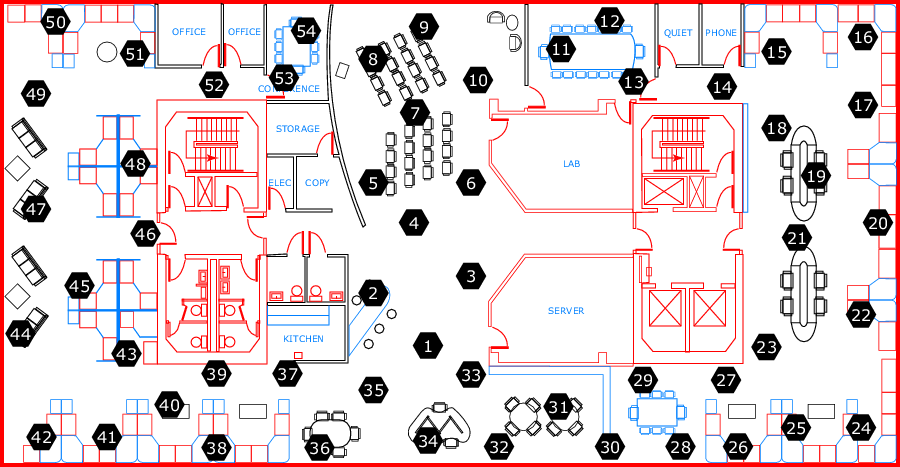
\includegraphics[scale=0.25]{berkeley_lab.png}
\caption{Intel Berkeley Research Lab Floorplan} \label{berkeley_lab}
\end{figure}

\paragraph*{Traffic Dataset}

The Traffic Dataset records the temperature, humidity, and voltage conditions of 20 sensor nodes and one gateway node.
This dataset, collected by the Bio-industrial Department at National Taiwan University, was recorded over a 2.5 year time period ending in 2011 in an outdoor location high traffic area in Taipei, Taiwan. \redtext{Include citation for Traffic Dataset! (Chun contacting authors)}

\begin{figure}[H]
\centering
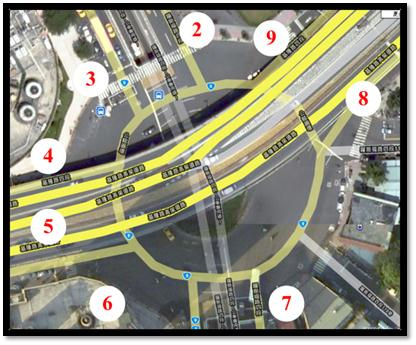
\includegraphics[scale=0.5]{traffic_wsn.png}
\caption{Traffic Sensor Deployment Configuration (7 sensors of 20 shown)}
\end{figure}

\subsubsection{Dataset Preparation}

\paragraph*{Berkeley Dataset Outlier Removal and Gridding}

Outlier Filtering : Observation removed if temperature $> 100\degc$, temperature $< 5\degc$, or humidity $< 16\%$.

Gridding : Dataset falls on even 30s intervals for the first 5000 time steps (which is all we consider), so no additional gridding need be performed.

\paragraph*{Traffic Dataset Outlier Removal and Gridding}

Outlier Filtering : Observation removed if temperature $< 5\degc$ or $> 60\degc$ or if humidity $< 10\%$ or $> 100\%$.

Gridding : The original dataset recorded most readings at around the $xx:03$ and $xx:33$ minute marks, so a $6$ min window centered at
these points captured the data for $30$ minute internal readings.
Where more than one reading was recorded for a given node within a given window, the closest to the $3$ or $33$ minute mark was chosen.
The full length of the dataset was used, which consists of $~43$K time-steps.

\paragraph*{Common Methodology}

%Datasets of various lengths are produced from the single input dataset for our experiments, namely 2500, 5000, and 10000.
There is an initially missing portion of the observations which can be considered Missing At Random (MAR).
To this, we impose two different types of Missing Completely At Random (MCAR) sampling techniques to build validation and testing datasets.

\paragraph*{Random Missing Pattern}

This pattern reflects choosing a random time and random sensor to be missing and hence removed from the training set.
We define two values $x$ and $y$ as follows.

\begin{itemize}
\item $10\%$ of the non-missing data is randomly selected (without replacement) to be the validation set
\item $y\%$ of the non-missing data is randomly selected (without replacement) to be the testing set
\item The remaining data is part of the training set (this would be $x\%$ of the total data given no missing; assuming missing rate of $m\%$, the actual data in training set is $90\%-x\%-m\%$
\end{itemize}

\paragraph*{Temporal Missing Pattern}

This pattern reflects testing the effect of all data missing after a certain point in time.
We define two values $x$ and $y$ as follows.

\begin{itemize}
\item Here, we have the last $y\%$ of time is in test and the prior $10\%$ to test is the validation.
\item The sensor node numbers ``covered up'' in the validation and testing for the Berkeley and Traffic datasets are ${4,19,45}$ and ${2,4,6,8,10,14,17,19,20,21}$, respectively.
Note that node $21$ of the Traffic dataset is the gateway node.
\end{itemize}
